\section{Method}
\label{sec:method}

\begin{figure}
	\centering
	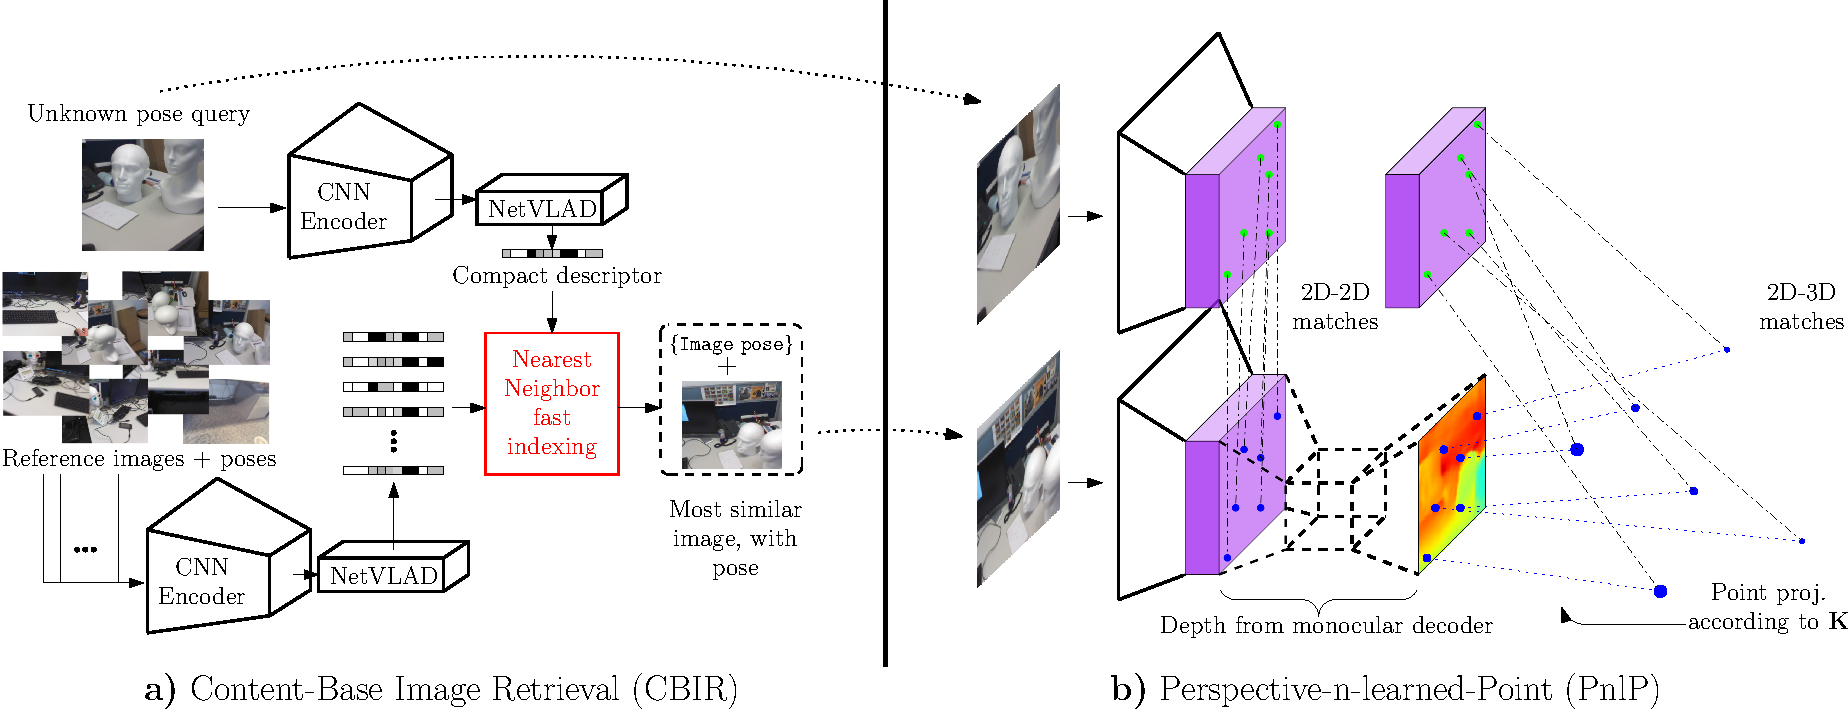
\includegraphics[width=\linewidth]{method/pipeline}	
	\caption[Pipeline of our pose refinement method]{\label{fig:pipeline} Pipeline of the proposed method. \textbf{a)} We retrieve initial pose of an image query using CBIR. \textbf{b)} We refine initial pose with a PnP algorithm where 2D to 3D matches are obtained through the reconstructed depth map of the reference image. \textcolor{purple}{Purple boxes} are deep features blocks used for dense images matching.}
\end{figure}


\paragraph{Workflow.}
Our method for fast image pose estimation is described in figure~\ref{fig:pipeline}. The camera pose is estimated following this two-step algorithm:
\begin{itemize}
	\item[\textbf{a)}] We obtain the initial pose of the query image by Content-Based Image Retrieval (section~\ref{subsec:image_indexing}).
	\item[\textbf{b)}] Initial pose is refined by finding dense correspondences between the query image and the best retrieved image (section~\ref{subsec:matching}). Meanwhile, we use a neural network to create the depth map related to the retrieved image candidate (section~\ref{subsec:depth_map}). We use correspondences between the 2D points of the query image and the 3D points projected from the depth map to compute the real pose of the query using Perspective-n-Point (PnP) algorithm (section \ref{subsec:pnlp}). We further denote our pose refinement method as Perspective-n-learned-Point (PnlP).
\end{itemize}

\paragraph{Notations.}
The aim of our method is to recover the camera pose $\mathbf{h_q}\in\mathbb{R}^{4\times 4}$, represented by a pose matrix in homogeneous coordinates, corresponding to an input RGB image $\mathrm{I_q}\in\mathbb{R}^{3\times H\times W}$. We know the matrix $\mathbf{K}\in\mathbb{R}^{3\times 3}$ of intrinsic parameters of the camera. We assume that we know the pose $\left\{ \mathbf{h_r}^{i} \right\}_{i=1,\ \ldots ,\ N}$ of a pool of $N$ references images $\left\{ \mathrm{I_{r}}^{i} \right\}_{i=1,\ \ldots ,\ N}$ of the scene where we want to localise the query. These poses can be obtained by Structure from Motion (SfM) or by using external sensors. We denote as $\mathrm{E}$, respectively $\mathrm{D}$, a neural network encoder, respectively decoder.

\subsection{Image retrieval}
\label{subsec:image_indexing}

We cast the initial pose estimation task as a content-based image retrieval problem like in~\cite{Balntas2018}, since the reference data are augmented with 6 DoF pose information. In order to evaluate the similarity between the unknown pose query image $\mathrm{I_{q}}$ and the $N$ reference images $\left\{\mathrm{I_{r}}^{i} \right\}_{i=1,\ \ldots ,\ N}$, we need to use a discriminative image representation. Recent works have shown that deep features extracted from convolutional neural network offer better global image representations compared to hand-crafted features~\cite{Razavian2014a, Arandjelovic2017, Gordo2017, Radenovic2017}. We use a state-of-the art global image descriptor for place recognition, NetVLAD~\cite{Arandjelovic2017}, to describe the data by low-dimensional $L_2$ normalized vectors. The NetVLAD descriptor $\mathbf{f}$ is obtained by concatenating the dense feature from neural network encoder $\mathrm{E}$: $\mathbf{f} = \mathrm{NetVLAD}(\mathrm{E}(\mathrm{I}))$.

We first compute reference descriptors $\left\{ \mathbf{f}_{\mathrm{r}}^{\ i} \right\}_{i=1,\ \ldots ,\ N}$ from the reference images. Then we compare the query descriptor $\mathbf{f}_{\mathrm{q}}$ to the pre-computed descriptors by fast nearest neighbor indexing and retrieval:
\begin{equation}
	\left\{ \mathbf{\hat{f}}_{\mathrm{r}}^{\ j} \right\}_{j=1,\ \ldots ,\ K} = NN \left( \mathbf{f}_{\mathrm{q}}, \left\{ \mathbf{f}_{\mathrm{r}}^{\ i} \right\}_{i=1,\ \ldots ,\ N} \right),
\end{equation}
where $NN$ is the nearest neighbor matching function and $\mathbf{\hat{f}}_{\mathrm{r}}^{\ j}, j \in [1, K]$, the $K$ closest reference descriptors to the query descriptor. We use cosine similarity to evaluate the similarity between two descriptors and K-D tree as indexing structure. We consider poses $\mathbf{h}_\mathrm{r}^j, j \in [1, K],$ as candidate poses of the image $\mathrm{I_q}$.

\subsection{Dense correspondences}
\label{subsec:matching}

In order to refine the initial pose obtained by image retrieval, we compute correspondences between the query image and the closest retrieved image candidates. In~\citep{Taira2018}, authors use the dense features extracted by a convolutional neural network in order to compute correspondences between images. We follow the same idea and use the latent representation already computed by the neural network encoder $\mathrm{E}$ to compute correspondences between the query image and the $K$ retrieved candidates.

Local image descriptors are obtained from the latent image representation by concatenating the features at each position $\left( l, m \right)_{W_\mathrm{E},H_\mathrm{E}}$ ($W_\mathrm{E}$ and $H_\mathrm{E}$ are the spatial dimensions of the features map) along the depth of the features map~\citep{Taira2018, Widya2018}. We subsequently $L_2$-normalize the extracted descriptors before matching. We consider only consistence matches by rejecting correspondences that do not respect the bidirectional test (nearest descriptors of image 1 in image 2 have to be the same as nearest descriptors of image 2 to image 1).

\subsection{Depth from monocular}
\label{subsec:depth_map}
2D to 2D correspondences obtained by dense features matching (section~\ref{subsec:matching}) do not provide enough information to compute relative pose between images at absolute scale. Therefore, we propose to reconstruct the relative scene geometry from the camera to circumvent this limitation. Various recent deep learning generative models are able to properly reconstruct geometry associated to radiometric data, with full supervision training~\cite{Eigen2014}, weakly annotated data~\cite{Godard2017} or even in a self-supervised way~\cite{Mahjourian2018}. 

We train an encoder/decoder jointly to predict the corresponding depth map $\mathrm{M}$ associated to an image: $\mathrm{M = D(E(I))}$. With the generated depth map obtained by our neural network and the intrinsic parameters of the camera $\mathbf{K}$, we can project the 2D point $\left( l, m \right)^T$ to the corresponding 3D coordinate $\mathbf{p}$:
\begin{equation}
	\label{eq:3d_proj}
	\mathbf{p} = \mathrm{M}^{l, m} \cdot \mathbf{K}^{-1}[l, m, 1]^T.
\end{equation}

\subsection{Pose refinement}
\label{subsec:pnlp}

Thanks to the generated depth map (section~\ref{subsec:depth_map}) and the equation~\ref{eq:3d_proj}, we can project 2D points from retrieved images into 3D coordinates. 2D-2D correspondences obtained in section~\ref{subsec:matching} can be interpreted as 2D-3D correspondences and we can use PnP algorithm to compute the relative transformation $\mathbf{h}_\mathrm{r \rightarrow q}$ between the query image and the reference image. Final pose of query image $\mathrm{I_q}$ is obtained with the equation:
\begin{equation}
	\mathbf{h}_\mathrm{q} = \mathbf{h}_\mathrm{r}\mathbf{h}_\mathrm{r \rightarrow q}.
\end{equation}

We embed the PnP algorithm within a RANSAC consensus where a sub-part of 2D-3D correspondences are evaluated at a time. As we have multiple reference candidates from image retrieval step (section~\ref{subsec:image_indexing}), we select the pose with the largest proportion of inlier correspondences after the PnP optimizationn. If the ratio of inlier is below a given threshold, we simply affect the pose of the retrieved image to the query.

\subsection{System design and motivation}
\paragraph{Multi-task model.} In order to make our system fast and lightweight, we use a single encoder/decoder neural network for the three tasks needed in our pose estimation pipeline. That means with a single image forward, we obtain a compact global image description, dense local descriptors and a depth map corresponding to the observed scene.
\paragraph{Single task training policy.} It exists in the literature methods for training deep neural network either for global image description~\citep{Arandjelovic2017, Radenovic2017, Gordo2017}, local features extraction and description~\citep{Yi2016a, Rocco2018, Ono2018} or depth from monocular estimation~\citep{Eigen2014, Godard2017, Mahjourian2018}. We decide to train our encoder/decoder network for the task of depth from monocular estimation because estimation of erroneous depth measurement will result in wrong estimation of the final pose. In the next section, we experimentally show that even if our network has not been trained especially for the task of image description or local feature matching, the latent features computed within the network embed enough high-level semantic to perform well on these tasks~\citep{Taira2018, Zamir2018}.
\paragraph{Generalisation.} Because we rely on a non-absolute representation of the scene geometry (depth is estimated \textit{relatively} to the camera frame), our model is not limited to localization on one specific scene like end-to-end pose estimation networks~\citep{Kendall2017, Brachmann2017b}. The same trained network can be used to localize images in multiple indoor and outdoor scenes, and even on totally unknown environments. 